\chapter{Описание предметной области}

Предметная область работы связана с учетом SIM-карт и телефонных номеров у мобильного оператора. В реальной работе оператор должен знать, какие номера свободны, какие уже выданы абонентам, какие SIM-карты находятся на складе, какие заблокированы и какие действия выполнялись сотрудниками.

Главный бизнес-процесс в такой системе это выдача номера абоненту. При выдаче сотрудник выбирает абонента, телефонный номер, SIM-карту и тариф. После этого в базе появляется запись о выдаче. Если номер нужно заблокировать, например из-за потери телефона или задолженности, создается запись о блокировке. Все важные действия сохраняются в истории операций.

\section{Основные сущности}

Для базы данных были выбраны восемь таблиц. Такой набор таблиц позволяет разделить данные по смыслу и не хранить разные сущности в одной общей таблице.

\begin{longtable}{|p{0.28\textwidth}|p{0.64\textwidth}|}
\caption{Назначение таблиц базы данных} \\
\hline
\textbf{Таблица} & \textbf{Назначение} \\
\hline
\endfirsthead
\hline
\textbf{Таблица} & \textbf{Назначение} \\
\hline
\endhead
\texttt{subscribers} & Хранит абонентов. В таблице есть ФИО, паспорт, почта, дата создания и статус абонента. \\
\hline
\texttt{tariffs} & Хранит тарифные планы. Для каждого тарифа указана абонентская плата, интернет, минуты и SMS. \\
\hline
\texttt{employees} & Хранит сотрудников, которые оформляют выдачи, блокировки и другие операции. \\
\hline
\texttt{phone\_numbers} & Хранит телефонные номера. У каждого номера есть регион и статус. \\
\hline
\texttt{sim\_cards} & Хранит SIM-карты. Для каждой SIM-карты указаны ICCID, IMSI, статус и дата поступления. \\
\hline
\texttt{number\_assignments} & Хранит факты выдачи номера абоненту. Это центральная таблица, которая связывает абонента, номер, SIM-карту, тариф и сотрудника. \\
\hline
\texttt{block\_requests} & Хранит блокировки и разблокировки. В таблице указывается причина, дата блокировки, дата разблокировки и статус. \\
\hline
\texttt{operation\_history} & Хранит журнал операций. В него записываются выдачи, блокировки, разблокировки, смены тарифа и закрытия выдач. \\
\hline
\end{longtable}

\section{Почему выбрана такая структура}

Таблица \texttt{number\_assignments} сделана центральной, потому что в задаче важно хранить не только сами номера и SIM-карты, но и факт их выдачи конкретному абоненту. Один номер может быть когда-то закрыт и потом выдан другому абоненту, поэтому выдача хранится отдельной записью.

Абоненты, номера, SIM-карты, тарифы и сотрудники вынесены в разные таблицы. Это сделано для нормализации данных. Например, название тарифа и его стоимость не нужно повторять в каждой выдаче. Достаточно хранить тариф один раз в таблице \texttt{tariffs}, а в выдаче записывать только ссылку на него.

Блокировки вынесены в отдельную таблицу, потому что у одной выдачи может быть несколько блокировок за все время обслуживания. История операций также выделена отдельно, чтобы можно было проследить действия сотрудников и восстановить последовательность событий.

\section{ER-диаграмма}

Логическая структура базы данных показана на рисунке 1. На диаграмме видно, что большинство связей идет через таблицу \texttt{number\_assignments}. Это удобно, потому что именно выдача объединяет абонента, номер, SIM-карту, тариф и сотрудника.

\begin{figure}[H]
    \centering
    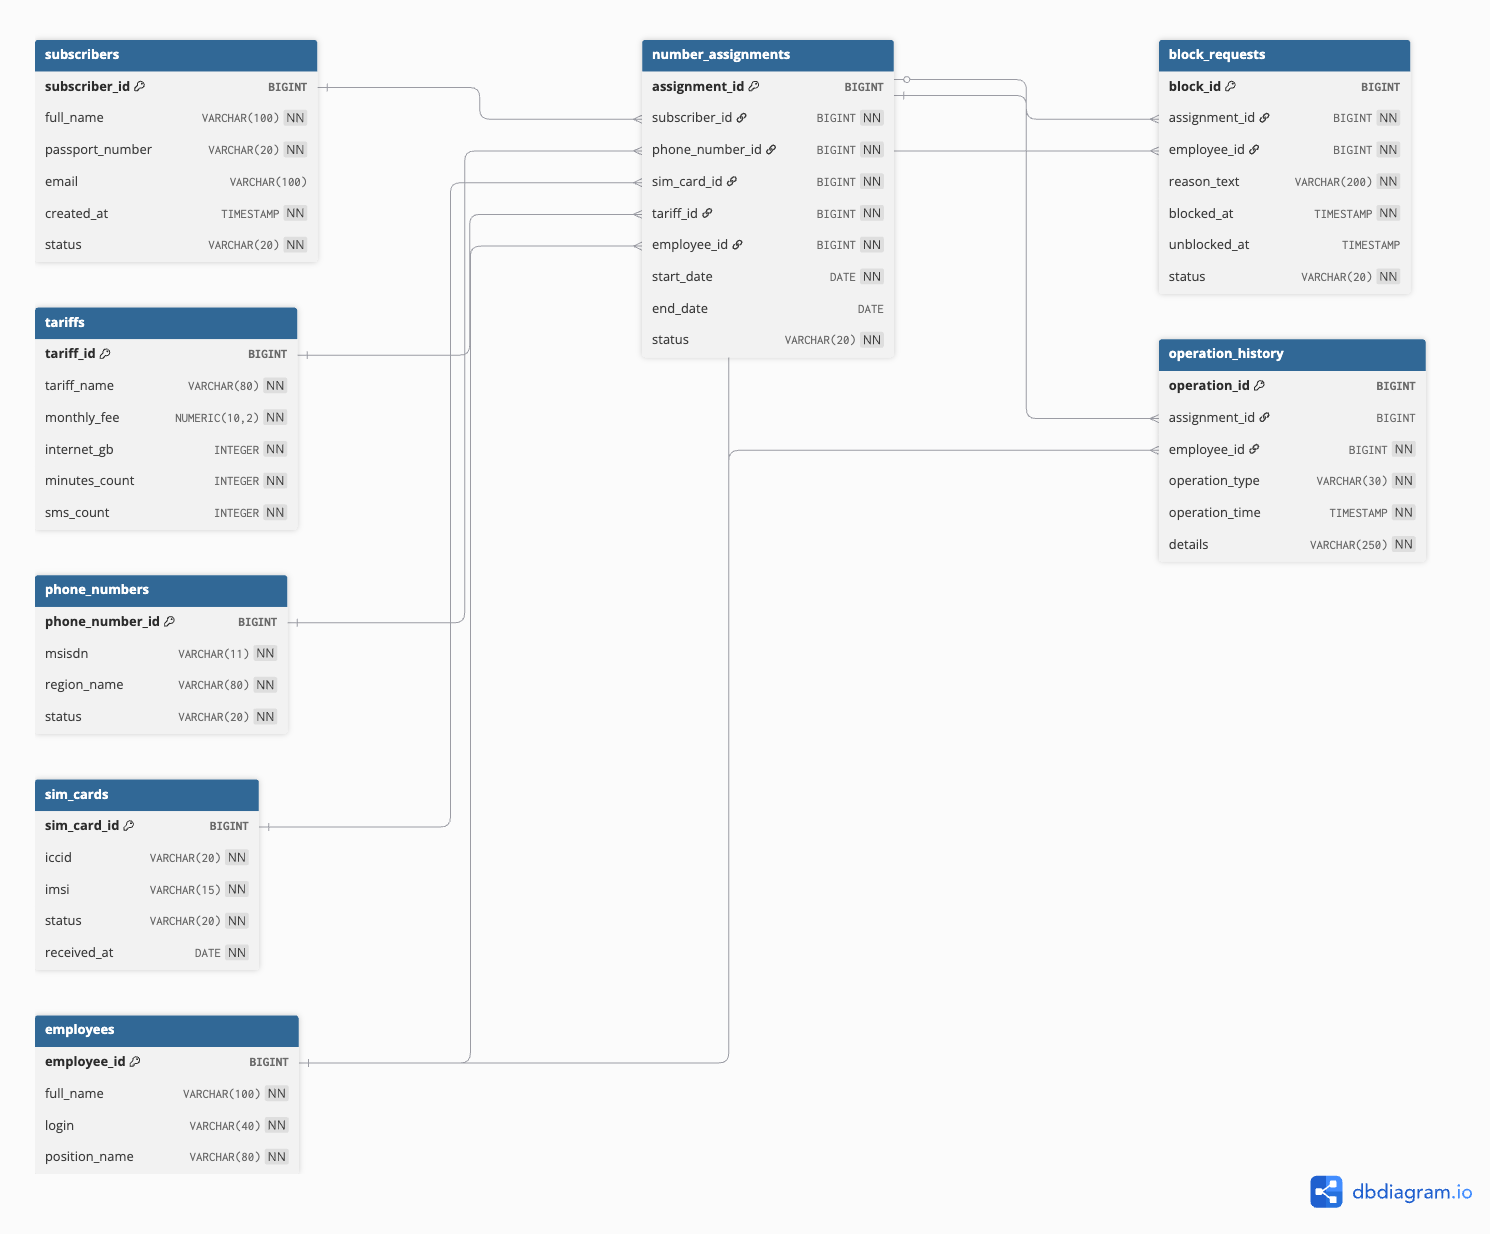
\includegraphics[width=\textwidth]{diagram_report.png}
    \caption{ER-диаграмма базы данных управления SIM-картами и номерами}
\end{figure}
